\documentclass[11pt,a4paper]{article}
\usepackage[top=3cm, bottom=2cm, left=2cm, right=2cm]{geometry}
\usepackage[utf8]{inputenc}
\usepackage{amsmath, amsfonts, amssymb}
\usepackage{siunitx}
\usepackage[brazil]{babel}
\usepackage{graphicx}
\usepackage[margin=10pt,font={small, it},labelfont=bf, textfont=it]{caption}
\usepackage[dvipsnames, svgnames]{xcolor}
\DeclareCaptionFont{MediumOrchid}{\color[svgnames]{MediumOrchid}}
\usepackage[pdftex]{hyperref}
\usepackage{natbib}
\bibliographystyle{plainnat}
\bibpunct{\textcolor{MediumOrchid}{\textbf{[}}}{\textcolor{MediumOrchid}{\textbf{]}}}{,}{s}{}{}
\usepackage{color}
\usepackage{footnote}
\usepackage{setspace}
\usepackage{booktabs}
\usepackage{multirow}
\usepackage{subfigure}
\usepackage{fancyhdr}
\usepackage{leading}
\usepackage{indentfirst}
\usepackage{wrapfig}
\usepackage{mdframed}
\usepackage{etoolbox}
\usepackage[version=4]{mhchem}
\usepackage{enumitem}
\usepackage{caption}
\usepackage{titlesec}
\usepackage{tcolorbox}
\usepackage{tikz}
\usepackage{LobsterTwo}
\usepackage[T1]{fontenc}
\usepackage{fontspec}
\usepackage{txfonts}
\usepackage[bottom]{footmisc}
\tcbuselibrary{skins,breakable}
\sisetup{output-decimal-marker={.}}

\makeatletter
\def\footnoterule{\kern-3pt\color{MediumOrchid}\hrule\@width0.6\textwidth height 0.8pt\kern2.6pt}
\makeatother

\renewcommand{\footnotelayout}{\itshape\color{MediumOrchid}}

\AtBeginEnvironment{equation}{\fontsize{13}{16}\selectfont}


\titleformat{\section}{\LobsterTwo\LARGE\color{CarnationPink}}{\thesection.}{1em}{}
\titleformat{\subsection}{\LobsterTwo\LARGE\color{CarnationPink}}{\thesubsection}{1em}{}
\titleformat{\subsubsection}{\LobsterTwo\large\color{MediumOrchid}}{\thesubsubsection}{1em}{}


\DeclareCaptionLabelFormat{figuras}{\textcolor{DarkTurquoise}{Figura \arabic{figure}}}
\captionsetup[figure]{labelformat=figuras}

\makeatletter
\renewcommand\tagform@[1]{\maketag@@@{\color{CarnationPink}(#1)}}
\makeatother

\renewcommand{\theequation}{Eq. \arabic{equation}}
\renewcommand{\thefigure}{Fig. \arabic{figure}}
\renewcommand{\thesection}{\textcolor{CarnationPink}{\arabic{section}}}

\setlist[itemize]{label=\textcolor{CarnationPink}{$\blacksquare$}}

\setlist[enumerate]{label=\textcolor{CarnationPink}{\arabic*.}, align=left, leftmargin=1.5cm}


\newcounter{exemplo}

\NewDocumentEnvironment{exemplo}{ O{} }{%
\allowbreak
\setlength{\parindent}{0pt}
  \begin{mdframed}[
  leftline=true,
  topline=false,
  rightline=false,
  bottomline=false,
  linewidth=2pt,
  linecolor=CarnationPink,
  frametitlerule=false,
  frametitlefont=\LobsterTwo\large\color{CarnationPink},
  frametitle={\color{CarnationPink}\LobsterTwo\large #1},
  ]
}{%
  \end{mdframed}
}

\setlength{\fboxsep}{5pt}
\setlength{\fboxrule}{1.5pt}
\usepackage{float}
\renewcommand{\thefootnote}{\alph{footnote}}
\usepackage{url}
\hypersetup{
	colorlinks=true,
	linkcolor=DarkTurquoise,
	filecolor=DarkTurquoise,      
	urlcolor=DarkTurquoise,
	citecolor=DarkTurquoise,
	pdftitle={Especialista em Física da Radioterapia}
}
\pagestyle{fancy}
\fancyhf{}
\renewcommand{\headrulewidth}{0pt}
\rfoot{Página \thepage}

\title{\LobsterTwo\Huge{Dosimetria}}
\author{\LobsterTwo\Large{Grandezas E Quantidades Dosimétricas\nocite{*}}}
\date{\LobsterTwo\textit{Dalila Mendonça}}
\begin{document}
	\maketitle

    As grandezas relacionadas a Dosimetria das Radiações auxiliam na determinação quantitativa da energia depositada pela radiação no meio. 
    
    
    \section{Fluência e Fluência de Energia dos Fótons}

        Embora seja definida para fótons, a fluência pode ser utilizada em partículas carregadas. 

        \

        A \textit{\textbf{\textcolor{MediumOrchid}{Fluência de Partículas $\mathbf{\Phi}$}}} é dado pela taxa de variação do número de partículas $dN$ incidentes em uma esfera com área de seção transversal $dA$, ou seja:

			\begin{equation}
			\Phi  = \frac{d N}{d A} 
			\end{equation}
		
		\begin{exemplo}[Unidade]
			\begin{itemize}
				\item A unidade de medida da fluência da partículas	\textcolor{DarkTurquoise}{[$\Phi =$]  \unit{m^{-2}}.}
			\end{itemize}
		\end{exemplo}


    	\noindent  O motivo por considerar apenas uma esfera com seção transversal $dA$ está relacionado ao fato de que só é considerado para a fluência uma área perpendicular a direção de propagação do feixe (uma vez que independente da angulação que o feixe está incidindo, sempre atravessará a mesma área transversal de uma esfera) e portanto não há dependência angular na fluência. Ao considerar uma fluência planar, será avalido o número de fótons que atravessam um plano por unidade de área, e portanto a fluência irá depender do ângulo de incidência do feixe. 

      	\

      	A \textit{\textbf{\textcolor{MediumOrchid}{Fluência de Energia $\mathbf{\Psi}$}}} E a razão entre a Energia Radiante Incidente ($dE$) e a área transversal de uma esfera ($dA$), ou seja:

			\begin{equation}
			\Psi = \frac{d E}{d A}
			\end{equation}


		\begin{exemplo}[Unidade]
			\begin{itemize}
				\item A unidade de medida da fluência de Energia é \textcolor{DarkTurquoise}{\unit{J \cdot m^{-2}}}.
			\end{itemize}
			
		\end{exemplo}

      	\noindent  A Fluência de energia pode ser calculada através da Fluência de partículas através da relação:

			\begin{equation}
			\Psi = \frac{d N}{d A} \cdot E = \Phi \cdot E
			\end{equation}
      
      	\noindent onde $E$ é a energia da partícula e $\Phi$ é o número de partículas com energia E, caracterizada por um feixe monoenergético. 

    	\

    	A maior parte dos feixes de fótons e de outras partículas são polienergéticos, e portanto para estes feixes são utilizados o \textit{\textbf{\textcolor{MediumOrchid}{Espectro de Fluência de Partículas $\Phi_E(E)$ e o Espectro de Fluência de Energia $\Psi_E(E)$}}}, onde:

			\begin{equation}
			\Phi_E(E) = \frac{d \Phi}{dE}(E)
			\end{equation}

      	\noindent e

			\begin{equation}
			\Psi_E(E) = \frac{d \Psi}{d E}(E) = \frac{d \Phi}{dE}(E) \cdot E 
			\end{equation}

		\

		A \textit{\textbf{\textcolor{MediumOrchid}{Taxa De Fluência Da Partícula}}} é dada pela taxa de variação da fluência em relação ao tempo, ou seja:

			\begin{equation}
				\dot{\Phi} = \frac{d \Phi}{d t}
			\end{equation}

		\noindent no qual é dada em \textcolor{DarkTurquoise}{\unit{m^{-2} \cdot s^{-1}}}.

		\

		A \textit{\textbf{\textcolor{MediumOrchid}{Taxa de Fluência de Energia}}}, também chamada de intensidade, é dada pela taxa de variação da fluência de energia em função do tempo, ou seja:

			\begin{equation}
				\dot{\Psi} = \frac{d \Psi}{d t}
			\end{equation}
		

		\begin{exemplo}[Unidade]
			\begin{itemize}
				\item A unidade de medida da Taxa de Fluência de Energia é \textcolor{DarkTurquoise}{\unit{W \cdot m^{-2}}} ou \textcolor{DarkTurquoise}{\unit{J \cdot m^{-2} \cdot s^{-1}}}.
			\end{itemize}
			
		\end{exemplo}
		
		
	\section{Exposição}

		A \textit{\textbf{\textcolor{MediumOrchid}{Exposição ($X$)}}} é a habilidade dos fótons ionizar o ar, dada pela seguinte  :

			\begin{equation}
				X = \frac{\Delta Q}{\Delta m_{ar}}
			\end{equation}

		\noindent onde $\Delta Q$ é o valor absoluto da carga total dos íons de um sinal produzidos no ar, quando todos os elétrons e pósitrons liberados ou criados por fótons em  massa de ar $\Delta m_{ar}$ são completamente parados no ar.
		
		\
		
		\begin{exemplo}[Unidade]

			\begin{itemize}
				\item A unidade de medida no SI é \textcolor{DarkTurquoise}{\unit{C \cdot Kg^{-1}}};
				\item  A unidade antiga da Exposição é o Roentgen (R) onde:

				\begin{equation*}
					1 R = 2.58 \times 10 ^{-4}\frac{C}{Kg}
				\end{equation*}
	
			\noindent porém está unidade já não é tão utilizada e portanto a unidade para Exposição é de textcolor{DarkTurquoise}{\qty{2.58e{-4}}{C/Kg}} de ar.
			\end{itemize}
			
		\end{exemplo}
		

	\section{Kerma}

		KERMA é o acrônimo para Energia Cinética Liberada Por Unidade de Massa. É uma quantidade não estocástica aplicável às \textcolor{MediumOrchid}{\textbf{radiações indiretamente ionizantes}}, como prótons e nêutrons. Esta grandeza quantifica a quantidade média de energia transferida pela radiação indiretamente ionizante para radiações diretamente ionizantes, sem se preocupar com o que acontece após esta transferência de energia. 

		Considerando os fótons, o processo de ionização se dá por duas etapas: 

			\begin{enumerate}[label=\textcolor{CarnationPink}{\arabic*${}^\circ$}]
				\item Os fótons transferem sua energia para as partículas carregadas secundárias, como os elétrons, por meio de diferentes processos de interação (Efeito Fotoelétrico, Efeito Compton, Produção de pares, etc \dots).
				
				\item A partícula secundária liberada irá então transferir sua energia através de processos como excitação e ionização. 
			\end{enumerate}

		O KERMA é então definido como a energia média transferida $d\bar{E}_{tr}$ de uma partícula indiretamente ionizante para partículas carregadas em um meio de massa $dm$, ou seja:

			\begin{equation}
				K = \frac{d \bar{E}_{tr}}{d m}
			\end{equation}
		
		\begin{exemplo}[Unidade]
			\begin{itemize}
				\item A unidade para o KERMA é de \textcolor{DarkTurquoise}{\unit{J \cdot Kg^{-1}}}.
			\end{itemize}
		\end{exemplo}
		


	\section{Dose Absorvida}

		A Dose absorvida é uma grandeza não-estocástica aplicável tanto para radiações indiretamente ionizantes quanto para radiações diretamente ionizantes. Para a radiação indiretamente ionizante, parte da sua energia é transferida como energia cinética para as partículas carregadas do meio, resultando no KERMA, e na sequência, as partículas carregadas perdem parcelas de sua energia para o meio, resultando na dose absorvida, e perdem parte da sua energia através da produção radiativa, em processos de bremmstrahlung ou aniquilação em voo. 
		
		
		A Dose  Absorvida está relacionada à uma quantidade estocástica chamada de energia transmitida ($\varepsilon$). A dose absorvida é definida como a energia média transmitida ($d\bar{\varepsilon}$) pela radiação \textcolor{MediumOrchid}{\textbf{diretamente ionizante}} para a matéria de massa $dm$ em um volume finito $V$, ou seja:


			\begin{equation}
				D = \frac{d \bar{\varepsilon}}{d m}
			\end{equation}

		\begin{exemplo}[Unidade]
			\begin{itemize}
				\item A unidade para a Dose Absorvida é o \textcolor{DarkTurquoise}{Gy = \unit{J \cdot Kg ^{-1}}}.
			\end{itemize}
		\end{exemplo}
		

		A energia transmitida $\varepsilon$ é a soma de todas as energias entrando no volume de interesse subtraída da soma de todas as energias que saem do volume de interesse, considerando qualquer conversão de massa-energia dentro do volume. \textcolor{MediumOrchid}{\textit{Por exemplo}},\textit{ a produção de pares diminui a energia em 1.022 MeV enquanto que a Aniquilação dos pares elétron-pósitron aumentam a energia pelo mesmo fator.}

		\textcolor{MediumOrchid}{\textit{\textbf{Obs:}}} Devido os elétrons viajarem no meio transferindo energia ao longo de sua trajetória, o local de deposição de energia é diferente do local onde a energia foi transferida pelo KERMA. 

		A \textbf{\textcolor{MediumOrchid}{Dose Equivalente $H_T$}} é dada por:

		\begin{equation}
			H_T = D_T \cdot w_R
		\end{equation}
	
		\begin{exemplo}[onde,]
			\begin{itemize}
				\item \textcolor{DarkTurquoise}{$\mathbf{D_T}$} é a dose média absorvida no órgão ou tecido;
				\item \textcolor{DarkTurquoise}{$\mathbf{w_{\text{R}}}$}  é o fator de ponderação da radiação.
				\item A unidade é  \textcolor{DarkTurquoise}{$\mathbf{Sv = (J/Kg)}$}
			\end{itemize}
		\end{exemplo}

		 A \ref{fig:fatorPesoRadiacao} mostra os valores para os fatores de ponderação fornecidos pela CNEN.

		\begin{figure}[h]
			\centering
			\fcolorbox{DarkTurquoise}{white}{%
			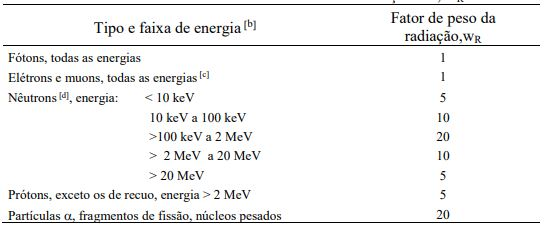
\includegraphics[width=0.8\textwidth]{Imagens/fatorPesoRadiacao.JPG}
			}%
			\caption{Fatores de ponderação para o tipo de radiação}
			\label{fig:fatorPesoRadiacao}
		\end{figure}


	\section{Stopping Power}

		O Stopping Power é definido através da teoria de Bethe para \textcolor{MediumOrchid}{\textbf{elétrons e pósitrons}}. É definido como o valor esperado da taxa de energia perdida por unidade de caminho percorrido para uma partícula carregada. O poder de freamento mássico divide o poder de freamento pela densidade do meio e elimina a dependência da densidade do meio no poder de freamento, exceto pelos efeitos de densidade. 

			\begin{exemplo}[Unidade]
				\begin{itemize}
					\item A unidade de medida do poder de freamento é \textcolor{DarkTurquoise}{$\mathbf{\unit{MeV/cm}}$}.
					\item A unidade de medida do poder de freamento mássico é \textcolor{DarkTurquoise}{$\mathbf{\unit{MeV/cm^2g}}$}.
				\end{itemize}
			\end{exemplo}

		Existem dois tipos de poder de freamento:

		\begin{enumerate}
			\item \textcolor{DarkTurquoise}{\textbf{Poder de Freamento de Colisão}}, também chamado de poder de freamento de ionização, onde é resultado das interações das partículas carregadas com os elétrons orbitais;
			\item \textcolor{DarkTurquoise}{\textbf{Poder de Freamento Radiativo}}, que é devido a interação das partículas carregadas com o núcleo do átomo.
		\end{enumerate}

		Além dos citados, o \textcolor{MediumOrchid}{\textbf{Poder de Freamento Mássico Irrestrito}} expressa a taxa média de perda de energia pela a partícula carregada devido às colisões duras e suaves. Neste caso, a energia máxima transferida para um elétron orbital permitida em uma colisão dura é igual a metade da energia cinética do elétron ou toda a energia de um pósitron. 


		O \textcolor{MediumOrchid}{\textbf{Poder de Freamento Mássico Restrito}} é definido para determinar a energia transferida localmente do meio por colisão, ou seja, não inclui a energia transferida para os raios delta que depositarão sua energia longe do local, e para isso determina-se um limiar de energia $\Delta$.

		O \textcolor{MediumOrchid}{\textbf{Poder de Freamento Linear por Colisão Restrito}}, também chamado de \textcolor{MediumOrchid}{\textbf{Transferência Linear de Energia (LET)}} é definido como a energia $dE_\Delta$ perdida por uma partícula carregada devido a colisões duras e suaves  ao atravessar uma distância linear $dl$ subtraída da energia cinética total das partículas carregadas liberadas cuja energia cinética excede o limiar $\Delta$.

			\begin{equation}
				L_\Delta = \frac{dE_\Delta}{dl}
			\end{equation}
	
		
	\section{Relação entre Fluência de Energia e Kerma (Fótons)}

		A energia transferida pelos fótons para os elétrons pode ser perdida através de interações por colisão (duras ou suaves) ou através de interações radiativas (bremsstrahlung e aniquilação de pares). 
		
		O Kerma total é dividido em duas partes:

		\begin{enumerate}
			\item \textcolor{DarkTurquoise}{\textbf{Kerma de Colisão:}} É a parte do kerma que leva a produção de elétrons que irão dissipar sua energia através ionizações causadas na trajetória ou nas proximidades da trajetória do elétron no meio, resultante da interação coulombiana com os elétrons orbitais. Portanto, kerma de colisão é o valor líquido de energia transferida para as partículas carregadas no ponto de interesse, excluindo a perda radiativa de energia e a energia transferida de uma partícula carregada para a outra.
			
			\item \textcolor{DarkTurquoise}{\textbf{Kerma Radiativo:}} É a parte do Kerma que leva à produção de fótons a medida que a partícula carregada é desacelerada e interage com o meio. A interação mais significativa é a radiação de freamento, porém também pode ser resultado da aniquilação em vôo.
		\end{enumerate}


		O \textcolor{DarkTurquoise}{\textbf{Kerma total $K$}} é então:

			\begin{equation}
				K = K_{col} + K_{rad}
			\end{equation}

		A fração média de energia transferida para os elétrons que é perdida através de processos radiativos é chamada de \textcolor{DarkTurquoise}{\textbf{fração radiativa $\bar{g}$}}. Portanto, a fração média de energia transferida para os elétrons que é perdida através de colisões é dada por $(1 - \bar{g})$ e o Kerma de colisão pode ser obtido através da seguinte equação:

			\begin{equation}
				K_{col} = K(1 - \bar{g})
			\end{equation}

		Para feixes monoenergéticos, a relação entre o Kerma de colisão e a fluência de energia $\Psi$ para um ponto no meio é dada por:

			\begin{equation}
				K_{col} = \Psi \left(\frac{\mu_{ab}}{\rho}\right)
			\end{equation}

		\noindent onde $\mu_{ab}/\rho$ é o coeficiente mássico de absorção de energia para feixes monoenergéticos. 

		Para feixes polienergéticos é considerado o espectro de energia, de forma que:

			\begin{equation}
				K_{col} = \int_{0}^{E_{max}} \Psi_E(E) \left(\frac{\mu_{ab}}{\rho}\right)  \,dE 
				= \Psi \left(\frac{\bar{\mu}_{ab}}{\rho}\right)
			\end{equation}

		\noindent onde:

			$$\Psi = \int_{0}^{E_{max}} \Psi_E(E) \, dE$$

		\noindent representa a fluência total de energia, e:

			$$\left(\frac{\bar{\mu}_{ab}}{\rho}\right)
			= \frac{1}{\Psi} \int_{0}^{E_{max}} \Psi_E(E) \left(\frac{\mu_{ab}}{\rho}\right)  \,dE
			$$

		\noindent é uma abreviação para o coeficiente mássico de absorção de energia para o meio calculado sobre o espectro de fluência de energia.


		Para feixes monoenergéticos, o Kerma total $K$ se relaciona com a fluência de energia $\Psi$ através da seguinte equação:

		\begin{equation}
			K = \Psi \left(\frac{\mu_{tr}}{\rho}\right)
		\end{equation}

		\noindent onde $\mu_{tr}/\rho$ é o coeficiente mássico de transferência de energia para feixes monoenergéticos. Semelhantemente ao Kerma de colisão, para feixes polienergéticos é considerado o espectro de fluência de energia para determinar o Kerma total.


		Dado dois meios com materiais diferentes, material 1 e material 2, a relação entre o Kerma de colisão destes materiais é obtida da seguinte forma:

		\begin{equation}
			\frac{K_{col,2}}{K_{col, 1}} = \frac{\Psi_2 \left(\frac{\mu_{ab}}{\rho}\right)_2}{\Psi_1 \left(\frac{\mu_{ab}}{\rho}\right)_1}
			\equiv \left(\Psi \right)_{2,1}\left(\frac{\mu_{ab}}{\rho}\right)_{2,1}
			\label{eq:razaoKcol}
		\end{equation}

		A   \ref{eq:razaoKcol} é frequentemente utilizada naquelas circunstâncias em que pode-se aproximar a razão entre as fluências de energia $(\Psi)_{2,1}$ para 1, que ocorre quando os materiais são muito similares ou quando a massa do material 2 é suficiente para fornecer um buildup (acúmulo) e ao mesmo tempo é pequena o suficiente de modo que não perturbe a fluência de fótons que atravessa o material 1.


	\section{Relação entre Fluência e Dose (Elétrons)}

		Dado as seguintes condições:

		\begin{enumerate}
			\item Os fótons produzidos no volume de interesse devido a produção radiativa, escapam do volume, ou seja, são espalhados para uma região distante do volume; e
			\item Os elétrons secundários liberados são absorvidos no local ou há um equilíbrio de partículas carregadas dos elétrons secundários.
		\end{enumerate}

		\noindent A \textbf{\textit{\textcolor{MediumOrchid}{Dose Absorvida}}} no meio $D_{m}$ está relacionada com a fluência eletrônica no meio $\Phi_{m}$ através da seguinte  :

			\begin{equation}
				D_m = \Phi_m \left(\frac{S_{col}}{\rho}\right)_m
				\label{eq:doseNoMeio}
			\end{equation}

		\noindent onde $(S_{col}/\rho)_m$ é o poder de freamento de colisão mássico irrestrito do meio.

		Devido a desaceleração do elétron no meio, mesmo para uma energia cinética inicial monoenergética $E_k$, sempre estará presente um espectro de fluência primário $\Phi_{m,E}$ que irá variar de $E_k$ até zero. Neste caso, a dose absorvida no meio pode ser obtida integrando a   \ref{eq:doseNoMeio}:

			\begin{equation}
				D_{m}= \int_{0}^{E_{max}} \Phi_{m, E}(E)\left(\frac{S_{col}}{\rho}\right)_{m}(E)  \,dE
				= \Phi_m \left(\frac{\bar{S}_{col}}{\rho}\right)_m
				\label{eq:doseAbsorvidaNoMeio}
			\end{equation}

		Desta forma, pode-se obter a dose absorvida através da fluência total de partículas e do poder de freamento de colisão médio para o espectro de energia das partículas carregadas. 

		A razão da dose absorvida entre o meio 1 e o meio 2, é dada por:

			\begin{equation}
				\frac{D_{m2}}{D_{m1}} = (\Phi)_{m2,m1} \left(\frac{\bar{S}_{col}}{\rho}\right)_{m2,m1}
			\end{equation}


		O espectro de fluência de elétrons realístico completo consiste nas partículas carregadas primárias, liberadas pelo feixes de fótons polienergéticos que interagiram com o meio, e que são desaceleradas, através das colisões duras e suaves, resultando em uma fluência de partículas carregadas secundárias (raios delta). 
		
		

	\section{Relação entre Kerma e Dose (Equilíbrio de Partículas Carregadas)}
		

		Geralmente, a transferência de energia do fóton para a partícula carregada em um determinado local não leva a absorção de energia pelo meio no mesmo local. Isto se deve ao alcance finito dos elétrons liberados através das interações dos fótons.

		Como os fótons secundários produzidos geralmente escapam do volume de interesse, a dose absorvida se relaciona principalmente com o Kerma de colisão; No entanto, a razão entre a dose e o kerma colisional é denotada por:

		\begin{equation}
			\beta = \frac{D}{K_{col}}
		\end{equation}

		\begin{wrapfigure}{r}{0.48\textwidth}
			\centering
			\fcolorbox{DarkTurquoise}{white}{%
			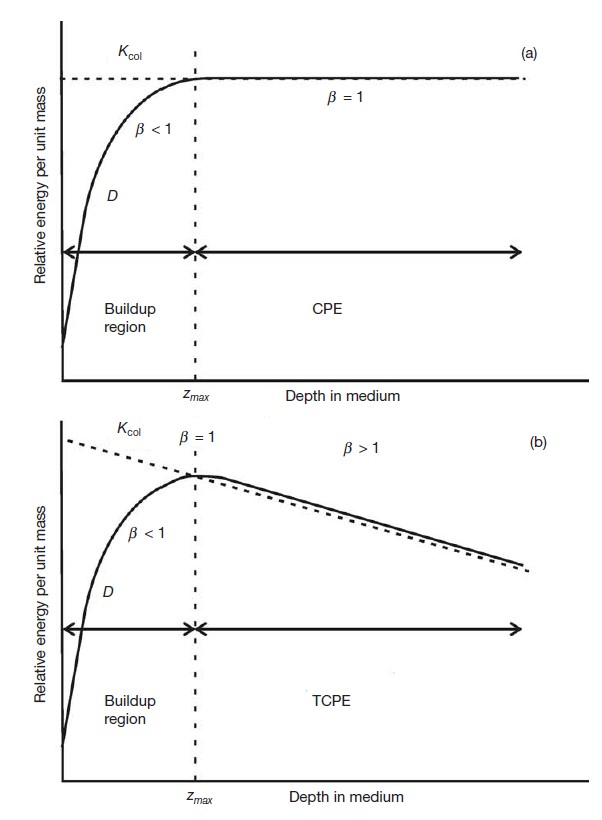
\includegraphics[width=0.43\textwidth]{Imagens/relacaoKermaEDose.jpg}
			}%
			\caption{Relação entre Dose Absorvida e Kerma}
			\label{fig:relacaoKermaEDose}
		\end{wrapfigure}
		
		A   \ref{fig:relacaoKermaEDose} mostra a relação entre o Kerma de colisão e a dose absorvida para um caso hipotético de equilíbrio de partículas carregadas (CPE) e para um caso de equilíbrio transiente de partículas carregadas (TCPE).

		A medida que um feixe de fótons de alta energia penetra no meio, o Kerma de colisão é máximo na superfície do material irradiado devido a fluência de fótons ser maior na superfície. Inicialmente, a fluência de partículas carregadas, e portanto a dose absorvida aumenta em função da profundidade até que a profundidade de dose máxima seja atingida.

		Considerando um caso hipotético no qual não houvesse atenuação ou espalhamento dos fótons no meio, mas ainda houvesse produção de elétrons, como mostra a   \ref{fig:relacaoKermaEDose}\textcolor{DarkTurquoise}{(a)}, ocorreria a região de buildup, onde $\beta < 1$ seguida por uma região de completo equilíbrio de partículas carregadas onde $\beta = 1$ e portanto $D = K_{col}$.

		Em uma situação realística, como apresentado na   \ref{fig:relacaoKermaEDose}\textcolor{DarkTurquoise}{(b)}, existe a atenuação e o espalhamento dos fótons no meio, fazendo com que ocorra uma região de equilíbrio transiente de partículas carregadas, onde existe uma relação aproximadamente constante entre o Kerma de Colisão e a dose absorvida. Esta relação é praticamente constante pois em feixes de fótons de alta energia, a energia média dos elétrons gerados e, portanto, seu alcance não tem mudança significativa com a profundidade do meio e portanto pode-se dizer que os elétrons são sempre liberados com a mesma energia.

		No caso especial em que existe equilíbrio de partículas carregadas, (na profundidade de dose máxima), a relação entre a dose absorvida D e o Kerma total K é dada por:

			\begin{equation}
				D = K_{col} = K(1 - \bar{g})
			\end{equation}

		\noindent onde $\bar{g}$ é a fração radiativa dependente da energia cinética do elétron e do meio. Quanto maior a energia cinética e maior o número atômico do meio, maior a fração $\bar{g}$.

		\begin{exemplo}[Exemplo]
			Para elétrons liberados em um meio de ar por um feixe de \ce{^{60}Co} a fração radiativa $\bar{g}$ é de 0.0032.
		\end{exemplo}

		O buildup da dose absorvida é responsável pelo efeito poupador da pele nos casos de irradiação com feixes de fótons de alta energia. Na prática, a dose na superfície é baixa mas não é nula devido a contaminação do feixe com elétrons devido a interação dos fótons com o meio acima do phantom, ou devido às partículas carregadas geradas no cabeçote do acelerador e nos dispositivos modificadores de feixe.

	\section{Relação entre Kerma e Exposição}

		A energia média liberada no ar por par de íons formados $W_{ar}$ é dada por:

			\begin{equation}
				W_{ar} = \frac{E_k}{N}
			\end{equation}

		\noindent onde N é o número médio de pares de íons formados quando a energia cinética inicial $E_k$ de uma partícula carregada é completamente dissipada no ar.

		\begin{exemplo}
			A melhor estimativa para o valor médio de $W_{ar}$ é de 33.97 eV/par de ions.

			\begin{equation}
				\frac{W_{ar}}{e} 
				= \frac{33.97 (eV/par)\times 1.602 \times 10^{-19} (J/eV)}{1.602 \times 10^{-19}(C/par)}
				= 33.97 \, J/C
			\end{equation}
		\end{exemplo}

		Multiplicando o Kerma de colisão por $(e/W_{ar})$, o número de coulombs de carga criada por joule de energia depositada, obtém-se a carga criada por unidade de massa de ar, ou seja, a exposição:

			\begin{equation}
				X = (K_{col})_{ar} \left(\frac{e}{W_{ar}}\right)
			\end{equation}

		E relação entre o Kerma total no ar e a exposição é dada por:

			\begin{equation}
				K_{ar} = X \left(\frac{W_{ar}}{e}\right) \frac{1}{1 - \bar{g}}
			\end{equation}

	\section{Teorias Cavitárias}

		Para medir a dose absorvida em um meio é necessário inserir um dosímetro neste meio com capacidade de medir a dose. Porém, o volume sensível deste dosímetro normalmente contém um material diferente daquele onde está inserido. Portanto, as teorias de cavidades relacionam a dose absorvida no volume sensível do detector (cavidade) com a dose absorvida no meio no qual a cavidade está inserida. 

		As teorias cavitárias são divididas com base no tamanho da cavidade, quando comparada ao alcance das partículas carregadas secundárias liberadas pelos fótons (  \ref{fig:teoriasDasCavidades}\textcolor{DarkTurquoise}{(a)}). Uma cavidade pequena é definida como uma cavidade que possui um diâmetro muito menor que o alcance dos elétrons liberados (\ref{fig:teoriasDasCavidades}\textcolor{DarkTurquoise}{(b)}); Uma cavidade intermediária possui um diâmetro da mesma ordem que o alcance dos elétrons secundários (\ref{fig:teoriasDasCavidades}\textcolor{DarkTurquoise}{(c)}); Já uma cavidade grande possui um diâmetro muito maior que o alcance dos elétrons liberados (\ref{fig:teoriasDasCavidades}\textcolor{DarkTurquoise}{(d)}). 

		\begin{figure}[h]
			\centering
			\fcolorbox{DarkTurquoise}{white}{%
			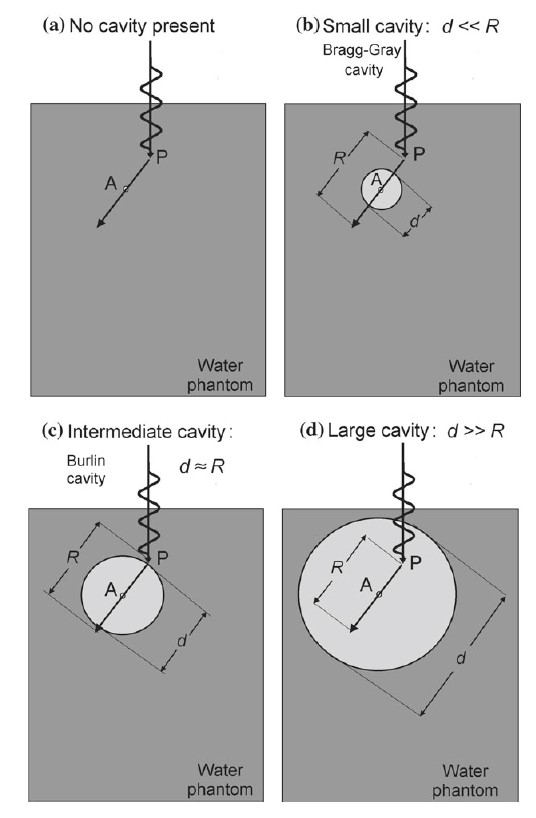
\includegraphics[width=0.5\textwidth]{Imagens/teoriasDasCavidades.jpg}
			}%
			\caption{Teorias Cavitárias}
			\label{fig:teoriasDasCavidades}
		\end{figure}

		
		\subsection*{Teoria Cavitária de Bragg-Gray}

			É a teoria utilizada nas pequenas cavidades, e pode ser utilizada quando as seguintes condições forem válidas:

			\begin{enumerate}[label=\textcolor{CarnationPink}{(\roman*)}]
				\item A cavidade deve ser pequena o suficiente quando comparada ao alcance das partículas carregadas que incidem na cavidade de forma que sua presença no meio não perturbe a fluência das partículas carregadas no meio;\label{cond:cav1}
				\item A dose absorvida na cavidade é depositada apenas pelas partículas carregadas que a atravessam, ou seja, as interações dos fótons na cavidade são desprezíveis de modo que possam ser ignoradas.\label{cond:cav2}
			\end{enumerate}


			A condição \ref{cond:cav1} implica que as fluências dos elétrons $\Phi_E(E)$ denotada na \ref{eq:doseAbsorvidaNoMeio} é a mesma e  igual à fluência de equilíbrio estabelecida no meio circundante. Esta condição só é válida em regiões onde ocorrem equilíbrio eletrônico ou de equilíbrio eletrônico transiente. Além disto, a presença de uma cavidade no meio sempre irá causar algum grau de perturbação na fluência de modo que é necessário introduzir fatores de correção para a perturbação.

			A condição \ref{cond:cav2} implica que todos os elétrons que depositam a dose dentro da cavidade são produzidos fora da cavidade e atravessam completamente a cavidade. Nenhum elétron secundário é, portanto, produzido dentro da cavidade e nenhum elétron irá parar completamente dentro da cavidade. 

			Sob estas duas condições, a Teoria cavitária de Bragg-Gray permite que a dose no meio $D_{meio}$ e a dose na cavidade $D_{cav}$ estão relacionadas a partir da seguinte  :

				\begin{equation}
					D_{meio} = D_{cav} \left(\frac{\bar{S}}{\rho}\right)_{meio, cav}
				\end{equation}

			\noindent onde $(\bar{S}/\rho)_{meio,cav}$ é a razão entre o poder de freamento de colisão mássico irrestrito do meio e da cavidade. O uso do poder de freamento irrestrito exclui a produção de partículas carregadas secundárias (raios delta) no meio e na cavidade.


			Embora o tamanho da cavidade não seja explicitamente levado em conta na teoria cavitária de Bragg-Gray, ele será fundamental para obedecer as duas condições estabelecidas. Portanto, uma cavidade que se qualifique como uma cavidade de Bragg-Gray para feixes de fótons de alta energia pode não se comportar como uma cavidade de Bragg-Gray para feixes de fótons de média e baixa energia.


		\subsection*{Teoria Cavitária de Spencer-Attix}

			A teoria cavitária de Bragg-Gray não considera os elétrons secundários (delta) gerados como resultado das colisões duras ocorridas durante o desaceleramento dos elétrons primários no volume sensível do dosímetro. A Teoria Cavitária de Spencer-Attix é uma formulação mais geral que considera a criação destes elétrons que possuem energia suficiente para causar suas próprias ionizações. 

			Alguns dos raios delta liberados dentro da cavidade preenchida com gás terão energia suficiente para sair da cavidade carregando parte de sua energia com eles. Este fato reduz a dose absorvida na cavidade e irá requerer uma modificação no poder de freamento do gás; 

			Portanto, a Teoria Cavitária de Spencer-Attix opera sob as mesmas condições estabelecidas para a Teoria Cavitária de Bragg-Gray com a diferença que estas condições serão aplicadas tanto para a fluência das partículas primárias quanto para a fluência das partículas secundárias.

			A fluência das partículas secundárias são divididas em duas componentes com base no limiar de energia $\Delta$ definido pelo usuário:

			\begin{enumerate}
				\item Elétrons secundários com energia cinética $E_K$ menor que $\Delta$, onde são considerados como elétrons lentos e irão depositar sua energia localmente e não participarão da fluência das partículas secundárias; e
				\item Elétrons secundários com energia cinética $E_K$ maior ou igual a $\Delta$, que são considerados rápidos e fazem parte do espectro dos elétrons. 
			\end{enumerate}

			Consequentemente, o espectro de partículas secundárias terá um limiar de baixa energia $\Delta$ e um limiar de alta energia $E_{K_0}$, onde $E_{K_0}$ representa a energia cinética inicial do elétron. Uma vez que a menor energia é $\Delta$, um elétron rápido com energia cinética $E_{K}$ maior ou igual a $2\Delta$ não poderá perder uma energia maior que $\Delta$; E um elétron rápido com energia cinética menor que $2\Delta$ não poderá perder uma energia maior que $E_K/2$, onde $(\Delta \leq E_K < 2\Delta)$. 

			Devido a Teoria Cavitária de Bragg-Gray que estipula que não deve haver a produção de elétrons dentro da cavidade, os elétrons com energia $\Delta$ devem ser capazes de atravessar a cavidade. O limar de energia $\Delta$ está então relacionado com o tamanho da cavidade e é definido como a energia do elétron com um alcance igual ao tamanho médio da linha ao longo da cavidade. 

			A relação entre a dose no meio e a dose na cavidade para a teoria cavitária Spencer-Attix é dada por:

				\begin{equation}
					\frac{D_{meio}}{D_{cav}} = s_{meio,cav}
				\end{equation}

			\noindent onde $s_{meio,cav}$ é a razão entre o poder de freamento de colisão mássico restrito do meio e da cavidade que é dado por:

			
			\begin{equation}
				s_{meio,cav}
				= \frac{\int_{\Delta}^{E_{K_0}} \Phi_{meio, E_k}^{e-e}(E_K)(L_{\Delta , meio}/\rho)\,dE_K + TE_{meio}}
				{\int_{\Delta}^{E_{K_0}} \Phi_{meio, E_k}^{e-e}(E_K)(L_{\Delta , cav}/\rho)\,dE_K + TE_{cav}}
			\end{equation}


			\begin{exemplo}[onde,]
				
			
			\begin{itemize}
				\item \textcolor{DarkTurquoise}{$(L_{\Delta}(E_K)/\rho)$} é o poder de freamento de colisão restrito com limiar de energia $\Delta$; \\
				\item \textcolor{DarkTurquoise}{$\Phi_{meio, E_k}^{e-e}(E_K)$} é a fluência de elétrons rápidos com energia variando de $\Delta$ até $E_{k_0}$.
				\item \textcolor{DarkTurquoise}{$e-e$} representa a contribuição de elétrons delta no espectro de desaceleração.
				\item \textcolor{DarkTurquoise}{$TE_{meio}$} e \textcolor{DarkTurquoise}{$TE_{cav}$} são chamados de termos de \textit{track end} e representam a parte da energia cinética depositada por elétrons com energia cinética inicial entre $\Delta$ e $2\Delta$ no meio e na cavidade, respectivamente. Estes elétrons podem ter uma perda de energia cinética que faz com que sua energia cinética fique menor que $\Delta$, de forma que sua energia residual após estes eventos seja depositada localmente e estes elétrons são removidos do espectro. 
			\end{itemize}
			\end{exemplo}

			Simulações de Monte Carlo mostram que existe uma diferença entre a Teoria de Bragg-Gray e a teoria de Spencer-Attix, mas que geralmente esta diferença não é muito significativa. Como os poderes de freamento colisional para diferentes meios mostram comportamentos semelhantes em função da energia, sua razão para os dois meios varia muito lentamente com a energia. 

			A razão entre o poder de freamento da água e do ar para as câmaras de ionização é fracamente dependente da energia de corte. Para câmaras de ionização tipo Farmer e câmaras de placas paralelas utilizadas em radioterapia o valor nominal para a energia de corte é normalmente de \qty{10}{keV}. Para uma câmara de ionização típica usada em água, a dependência energética da relação água/ar do poder de freameno surge principalmente da diferença na correção do efeito de densidade entre os dois materiais.


		\subsubsection*{Aplicação da Teoria Cavitária em Câmaras de Ionização}

			No contexto das teorias cavitárias, o volume sensível de um dosímetro é identificado como a cavidade, no qual pode estar preenchido com um gás, um líquido ou um sólido limitado por uma parede feita de outro material. Normalmente é utilizado gás pois permite um meio elétrico mais simples para a coleta de cargas liberadas no volume sensível pela radiação. 

			O meio que envolve a cavidade de uma câmara de ionização depende da situação em que o dispositivo é usado. Em uma abordagem mais antiga, a parede (geralmente suplementada com uma tampa de buildup) serve como meio de buildup e a teoria de Bragg-Gray fornece uma relação entre a dose no gás e a dose na parede. Isso é referido como uma câmara de ionização de paredes espessas e forma a base dos padrões de kerma no ar baseados em câmaras de cavidade e dos protocolos de dosimetria baseados em $C_\lambda$ da década de 1970. Se, no entanto, a câmara for usada em um fantoma sem a capa de buildup, uma vez que as espessuras típicas da parede são muito mais finas do que o alcance dos elétrons secundários, a proporção da dose da cavidade devido aos elétrons gerados no fantoma excede em muito a contribuição da dose na parede e, portanto, o fantoma serve como meio e a parede é tratada como uma perturbação nesse conceito.

			No caso de uma \textbf{\textcolor{MediumOrchid}{câmara de ionização de paredes espessas}} em um feixe de fótons de alta energia, a espessura da parede deve ser maior que o alcance dos elétrons secundários no material da parede para garantir que os elétrons que atravessam a cavidade surjam da parede e não do meio. A   da cavidade de Bragg-Gray então relaciona a dose na cavidade com a dose na parede da câmara. A dose no meio está relacionada com a dose na parede por meio de uma razão entre os coeficientes mássicos de absorção de energia do meio e da parede $(\bar{\mu}_{ab}/\rho)_{meio, wall}$, assumindo que:

			\begin{enumerate}
				\item A dose absorvida é igual ao Kerma de colisão; e
				\item A fluência dos fótons não é perturbada pela presença da câmara.
			\end{enumerate}

			A dose na cavidade de gás está relacionada com a ionização produzida na cavidade através da  :

				\begin{equation}
					D_{gas} = \frac{Q}{m}\left(\frac{\bar{W}_{gas}}{e}\right)
				\end{equation}

			\noindent onde $Q$ é a carga (de qualquer sinal) produzida na cavidade e $m$ é a massa de gás na cavidade.

			A teoria cavitária de Spencer-Attix pode ser utilizada para calcular a dose no meio através das seguintes relações:

			$$D_{meio} = D_{wall} \left(\frac{\bar{\mu}_{ab}}{\rho}\right)_{meio, wall} = D_{gas} s_{wall, gas}\left(\frac{\bar{\mu}_{ab}}{\rho}\right)_{meio, wall}$$

			\begin{equation}
				D_{meio} = \frac{Q}{m}\left(\frac{\bar{W}_{gas}}{e}\right)s_{wall, gas}\left(\frac{\bar{\mu}_{ab}}{\rho}\right)_{meio, wall}
				\label{eq:doseParedeEspessa}
			\end{equation}

			\noindent onde $s_{wall, gas}$ é a razão entre o poder de freamento de colisão mássico restrito da parede da cavidade e do gás com um limiar de energia $\delta$. Na prática, são adicionados fatores de correção à   \ref{eq:doseParedeEspessa} para satisfazer as condições 1 e 2 citadas acima.

			Uma   similar à   \ref{eq:doseParedeEspessa} é utilizada para as calibrações de Kerma no ar; no entanto a quantidade de interesse já não é mais a dose no meio e sim o Kerma no ar e portanto são introduzidos fatores de correção substanciais para a parede afim de garantir o completo equilíbrio eletrônico na parede e satisfazer a condição 1.

			No caso de uma \textbf{\textcolor{MediumOrchid}{câmara de ionização de paredes finas}} em um feixe de fótons ou elétrons de alta energia, a parede, a cavidade e o eletrodo central são tradados como uma perturbação na fluência do meio e a   envolve a razão entre os poderes de freamento restrito do meio e do gás da seguinte forma:

				\begin{equation}
					D_{meio} = \frac{Q}{m}\left(\frac{\bar{W}_{gas}}{e}\right)s_{meio, gas}\, p_{fl}\, p_{dis}\, p_{wall}\, p_{cel}
				\end{equation}

			\begin{exemplo}[onde,]
				\begin{itemize}
					\item \textcolor{DarkTurquoise}{$\mathbf{p_{fl}}$} é o fator de correção para a perturbação na fluência dos elétrons;
					\item \textcolor{DarkTurquoise}{$\mathbf{p_{dis}}$} é o fator de correção para o deslocamento do ponto efetivo de medida;
					\item \textcolor{DarkTurquoise}{$\mathbf{p_{wall}}$} é o fator de correção para a parede;
					\item \textcolor{DarkTurquoise}{$\mathbf{p_{cel}}$} é o fator de correção para o eletrodo central.
				\end{itemize}
			\end{exemplo}

  \bibliography{ref.bib}
\end{document}  